\documentclass[dutch, oneside]{tudelft-report}

\usepackage[utf8]{inputenc}
\usepackage{siunitx}
\usepackage{nameref}

\usepackage{verbatim}
%\usepackage[hidelinks]{hyperref}
\usepackage[dutch]{babel}
\usepackage{xcolor}
\usepackage{graphicx}
%\usepackage[table]{xcolor}
\usepackage{pdfpages}
%\usepackage{mathtools}
%\usepackage{hyperref}
\usepackage{cleveref}
\usepackage{longtable}			% Table is te groot
\usepackage{tikz}				% Voor fsm
\usepackage{listings}			% Used to include VHDL-code and fragments
\usepackage[dutch]{babel}		% Dutch hyphenation patterns and dutch names 
\usepackage{soul}				% dingen doorstrepen
\usepackage[normalem]{ulem}				%dingen dooruniten
\usepackage{pslatex}			% Times, helvetica and courier
\usepackage[T1]{fontenc}		% Nicer font-encoding
\usepackage{hyperref}			% Gives clickable references in pdf-file
\usepackage{graphicx}			% Used to include .pdf, .jpg and .png-files
\usepackage{tabularx}			% Used for evenly spread tables
\usepackage{eso-pic}			% Absolute positioning, used for lines-to-track appendix and front- and backpage
\usepackage{datetime}			% Used for some data-references
%\usepackage[font=small,format=plain,labelfont=bf,up,textfont=up]{caption}	% Nicer captions
\usepackage{nonfloat}			% Captions for non-floating figures and tables
\usepackage{nextpage}			% Advanced nextpage commands
\usepackage{keystroke}			% "real" keys
\usepackage[nottoc]{tocbibind}		% Include Bibliography in ToC
\usepackage{multirow}			% Span text over multiple rows
\usepackage{verbatim}			% For comment-environment
%\usepackage[left=3.5cm, right=2.5cm]{geometry}
\usepackage{enumitem} % Mogelijkheid tot geen enters in itemize en enurate

%\crefname{equation}{vergelijking}{vergelijkingen}
%\crefname{table}{tabel}{tabellen}
%\crefname{figure}{figuur}{figuren}


\definecolor{comment}{RGB}{0, 15 , 117}		%Kleur blauw defineren
\definecolor{keyword}{RGB}{165, 42, 42}		%Kleur rood defineren
\definecolor{STD}{RGB}{46, 139, 87}			%Kleur groen defineren
\lstdefinelanguage{VHDL}{
  morekeywords=[1]{ 		%Defineren van keywords die blauw worden
    library,use,all,entity,is,port,in,out,end,architecture,of,
    begin,and,or,not,downto,ALL,signal,type,case,if,elsif,for,when,array,
    others,loop,process,to
  },
  morekeywords=[2]{			%Defineren van keyword die groen worden
    STD_LOGIC_VECTOR,STD_LOGIC,STD_LOGIC_1164,
    NUMERIC_STD,STD_LOGIC_ARITH,STD_LOGIC_UNSIGNED,std_logic_vector,unsigned,
    std_logic
  },
  morecomment=[l]--
}
\lstdefinestyle{vhdl}{
  language     = VHDL,
  basicstyle   = \footnotesize \ttfamily,
  keywordstyle = [1]\color{keyword}\bfseries, %Keywords kleuren
  keywordstyle = [2]\color{STD}\bfseries,	%Keywords kleuren
  commentstyle = \color{comment}, % Commits kleuren
  numbers=left,					  % Regel nummering
  breaklines=true,                % sets automatic line breaking
  tabsize=4                       % sets default tabsize to 4 spaces
}

\begin{document}

%% Use Roman numerals for the page numbers of the title pages and table of
%% contents.
\frontmatter

\title[Title\\ Midterm report]{EPO-3}
\author{Projectgroep A1}
\affiliation{Technische Universiteit Delft} 
\coverimage{cover/Light-Bulb}
\makecover

%% Include an optional title page.
%\begin{titlepage}

\begin{center}

%% Insert the TU Delft logo at the bottom of the page.
\begin{tikzpicture}[remember picture,overlay]
    \node at (current page.south)[anchor=south,inner sep=0pt]{
        
\includegraphics{cover/logo}
    };
\end{tikzpicture}

%% Extra whitespace at the top.
\vspace*{2\bigskipamount}

%% Print the title in cyan.
{\makeatletter
\titlestyle\color{tudelft-cyan}\Huge\@title
\makeatother}

%% Print the optional subtitle in black.
{\makeatletter
\ifx\@subtitle\undefined\else
    \bigskip
    \titlefont\titleshape\LARGE\@subtitle
\fi
\makeatother}

\bigskip
\bigskip

by
%door

\bigskip
\bigskip

%% Print the name of the author.
{\makeatletter
\titlefont\Large\bfseries\@author
\makeatother}

\vfill

in partial fulfillment of the requirements for the degree of
%in overeenstemming met de vereisten voor het verkrijgen van de graad van

\bigskip
\bigskip

{\bfseries Master of Science}

in Applied Physics

\bigskip
\bigskip

at the Delft University of Technology,
%aan de Technische Universiteit Delft,

to be defended publicly on Tuesday January 1, 2013 at 10:00 AM.
%in het openbaar de verdedigen op dinsdag 1 januari om 10:00 uur.

\vfill

\begin{tabular}{lll}
%% Add additional information here, per faculty requirements, e.g
%    Student number: & 1234567 \\
%    Project duration: & \multicolumn{2}{l}{March 1, 2012 -- January 1, 2013} \\
    Supervisor: & Prof.\ dr.\ ir.\ A.\ Einstein \\
    Thesis committee:
        & Prof.\ dr.\ C.\ F.\ Xavier, & TU Delft \\
        & Dr.\ E.\ L.\ Brown, & TU Delft \\
        & Ir.\ M.\ Scott, & Acme Corporation
\end{tabular}

%% Only include the following lines if confidentiality is applicable.
\bigskip
\bigskip
\emph{This thesis is confidential and cannot be made public until December 31, 2013.}
%\emph{Op dit verslag is geheimhouding van toepassing tot en met 31 december 2013.}

\bigskip
\bigskip
An electronic version of this thesis is available at \url{http://repository.tudelft.nl/}.
%Een elektronische versie van dit verslag is beschikbaar op \url{http://repository.tudelft.nl/}.

\end{center}

\end{titlepage}

%\chapter*{Preface}
\setheader{Preface}

Preface\ldots

\begin{flushright}
{\makeatletter\itshape
    \@author \\
    Delft, January 2013
\makeatother}
\end{flushright}

\tableofcontents

%% Use Arabic numerals for the page numbers of the chapters.
\mainmatter 

\chapter{Samenvatting}
Dit is het verslag van "EPO-3" van groep A1. Hierin is te vinden hoe het project is aangepakt en uitgewerkt. Het systeem dat is ontworpen lijkt op de Wake-up Light van het bedrijf Philips. De opstakels die overwonnen moesten worden zijn het ontvangen en verwerken van het DCF-77 signaal, het aansturen van het licht, het aansturen van het geluid en het aansturen van een LCD schermpje. In het verslag is te vinden hoe al deze subsystemen zijn ontworpen en uitgewerkt. 

\chapter{Introductie}
Epo 3 staat in het teken van het ontwerpen van een chip. Wat voor product er ontworpen gaat worden ligt aan de projectgroep. Het bedenken van het ontwerp is de eerste stap in het ontwerpproces, bij deze stap moet er al rekening gehouden met de randvoorwaarden die aan het project gesteld worden, zoals het aantal beschikbare transistoren op de chip.\\
Er is besloten om een wake-up light te maken. De belangrijkste functie is dat het licht 15 minuten voor de alarmtijd langzaam aan begint te gaan, totdat de lamp op de alarmtijd op volle sterkte brandt. Daarnaast zullen er nog een paar functies toegevoegd worden. Het DCF-signaal zal opgevangen worden voor de actuele datum en tijd, dit zal op een LCD-scherm worden laten zien. Door middel van vijf knoppen kan de wekker bediend worden. De alarmtijd kan ingesteld worden en de gebruiker kan aangeven of het licht en geluid aan moeten gaan als de gebruiker gewekt wil worden. Op de LCD zal ook te zien zijn of er iets aangepast wordt. De ingangs- en uitgangssignalen en het gedrag moeten geformuleerd worden als specificaties.\\
Er wordt structuur aangebracht in het systeem door het systeem op te delen in een paar grote blokken, deze blokken kunnen dan over de acht projectleden verdeeld worden. Allereerst moeten er van de afzonderlijke subsystemen specificaties opgesteld worden, zodat de blokken op elkaar afgestemd kunnen worden. Vervolgens moet van elk blok \'e\'en of meer FSM's gemaakt worden waarna er een code geschreven kan worden. De geschreven code moet gesimuleerd en gesyntetiseerd worden. Als aan het eind van het project van het hele systeem een lay-out gemaakt is, kan het systeem op een chip gezet worden.


\chapter{Design specification}
Het systeem moet aan verschillende specificaties voldoen. Zo zal het een algemene reset moeten bevatten. Als gevolg van het indrukken van de resetknop zullen alle opgeslagen waarden en counters op 'nul' worden gezet. Ook zullen alle signalen 'active high' moeten zijn. De tijd, die intern wordt bijgehouden, zal worden gesynchroniseerd met een zogenaamd DCF signaal.\\
De wekker zal bediend worden door middel van een menu. dit menu word aangestuurd op basis van 4 knoppen. In dit menu moet de wekkertijd ingesteld moeten worden. Ook moet de wekker en het wekker geluid aan en uit gezet kunnen worden.\\
De visualisatie van dit menu zal op een LCD weergegeven worden. Als men zich niet in het menu bevindt, zal men alle data verdeeld over het scherm zien. Deze data bestaat uit de actuele tijd, de wekker tijd, de datum en de weekdag. Daarnaast zal op het LCD scherm weergegeven worden of de wekker en het geluid aan staan. Met het knipperen van scheidingsteken tussen uren en minuten zal het passeren van seconden aangegeven worden.\\
Het systeem zal de volgende ingangen hebben:
\begin{itemize}[nolistsep]
\item	DCF-signaal
\item	36kHz klok
\item	Reset-knop
\item	4 menu-knoppen
\end{itemize}

\noindent
\\
Onze chip zal over de volgende uitgangen beschikken:
\begin{itemize}[nolistsep]
\item	RGB, een 3-bits uitgang om de ledjes aan te sturen
\item	Sound, 1 bit om de buzzer aan te sturen
\item	LCD, een \# bits vector om het scherm aan te sturen
\item	DCF\_debug, bit om aan te geven of er een DCF-signaal ontvangen wordt.
\end{itemize}


\chapter{Design overview and system design}
text text text...

\chapter{DCF controller}
text text text...

\chapter{Main controller}
\section{Inleiding}
De main controller bevat de interface van de wekker. Deze zorgt er voor dat een wekker ingesteld kan worden, aangepast kan worden en uitgezet kan worden. Belangrijk aan elke interface is, dat deze gebruiksvriendelijk is. Dit kan onder andere bereikt worden door een optimum voor het aantal knoppen te bepalen. Te veel knoppen, en de gebruiker weet niet welke knop wat doet, te weinig knoppen, en de gebruiker moet navigeren door nodeloos ingewikkeld menu. \\
Daarnaast is er nog een beperkende factor: het aantal pinnen op de chip. \\
Al deze informatie samengenomen, is besloten dat 4 knoppen voor de interface het meest gebruiksvriendelijke resultaat oplevert. Daarnaast is er nog een knop die slechts gebruikt wordt om een afgaand alarm uit te zetten. \\
De controller stuurt een hoop dingen aan, en van te voren was al geanticipeerd dat dit hierdoor een van de grootste onderdelen van de chip zou kunnen worden.

\section{Specificaties}
\subsection{Ingangen}
\begin{itemize}[nolistsep]
\item Klok, dit is een standaard input;
\item Reset, ook dit is een standaard input;
\item Knoppen, dit zijn de 4 knoppen die (nadat ze gebufferd zijn) onderdeel zijn van de interface.
\begin{itemize}[nolistsep]
\item knoppen[0] = menu
\item knoppen[1] = set 
\item knoppen[2] = up
\item knoppen[3] = down\\
\end{itemize}
\end{itemize}



\subsection{Uitgangen}
\begin{itemize}[nolistsep]
\item Wekker, dit is de tijd dat de wekker af moet gaan en de wekkerdata, dus of het licht en geluid aan staan, en of de wekker uberhaupt aanstaat;
\item Menu-state, dit is de staat in welke de FSM zich op het moment bevindt. Deze informatie wordt doorgevoerd naar het LCD-scherm om zo te kunnen zien waar in het menu men zit.\\
\end{itemize}
In \cref{tab:uitgangen_controller} wat voor informatie te vinden is in de uitgangen van de controller.
\begin{table}[ht!]
\begin{tabular}{|l|p{10cm}|}
\hline
Uitgang & Informatie over wat in de uitgang te vinden is \\ \hline
wekdata & De huidige info over de wekker instellingen uit geheugen \newline
wekdata[5 down to 0] daarin staan de minuten \newline
wekdata[10 down to 6] daarin staan de uren \newline
wekdata[11] geluid bit \newline
wekdata[12] led bit \newline
wekdata[13] wekker bit (Of de wekker uberhaupt aan is of niet) \\ \hline
menu & Deze geeft door aan de in welke state we zitten aan de lcd module \newline
000 : Het normale scherm weergeven met alarm en wekkertijd weergave state: Rust,Wekkertijd \newline
001 : Uren aanpassen \newline
010 : Minuten aanpassen \newline
011 : Led aanpassen \newline
100 : Geluid aanpassen \\ \hline
\end{tabular}
\caption{Uitgangen van de controller}
\label{tab:uitgangen_controller}
\end{table}
\newpage
\subsection{Gedrag}
Om te beginnen moet de tijd waarop de wekker af moet gaan ingesteld kunnen worden. Dit wordt gedaan door eerst de huidige wekkertijd weer te geven, vervolgens het uur waarop gewekt moet worden te wijzigen en daarna de minuut. Hierna wordt de huidige tijd weer weergegeven. \\
Daarnaast is een vereiste dat de led uitgezet moet kunnen worden. Afhankelijk van een instelling moet het wake-up-light gedeelte wel of niet aangaan. Hetzelfde geld voor het geluid. \\
Dit alles moet zo gebruiksvriendelijk mogelijk gebeuren.

\section{Functionaliteit}

\subsection{FSM}
In \cref{fig:FSM_controller} staat de gemaakte fsm en in \cref{tab:states_controller} staan de uitgangen per state gespecificeerd.

\begin{figure}[ht!]
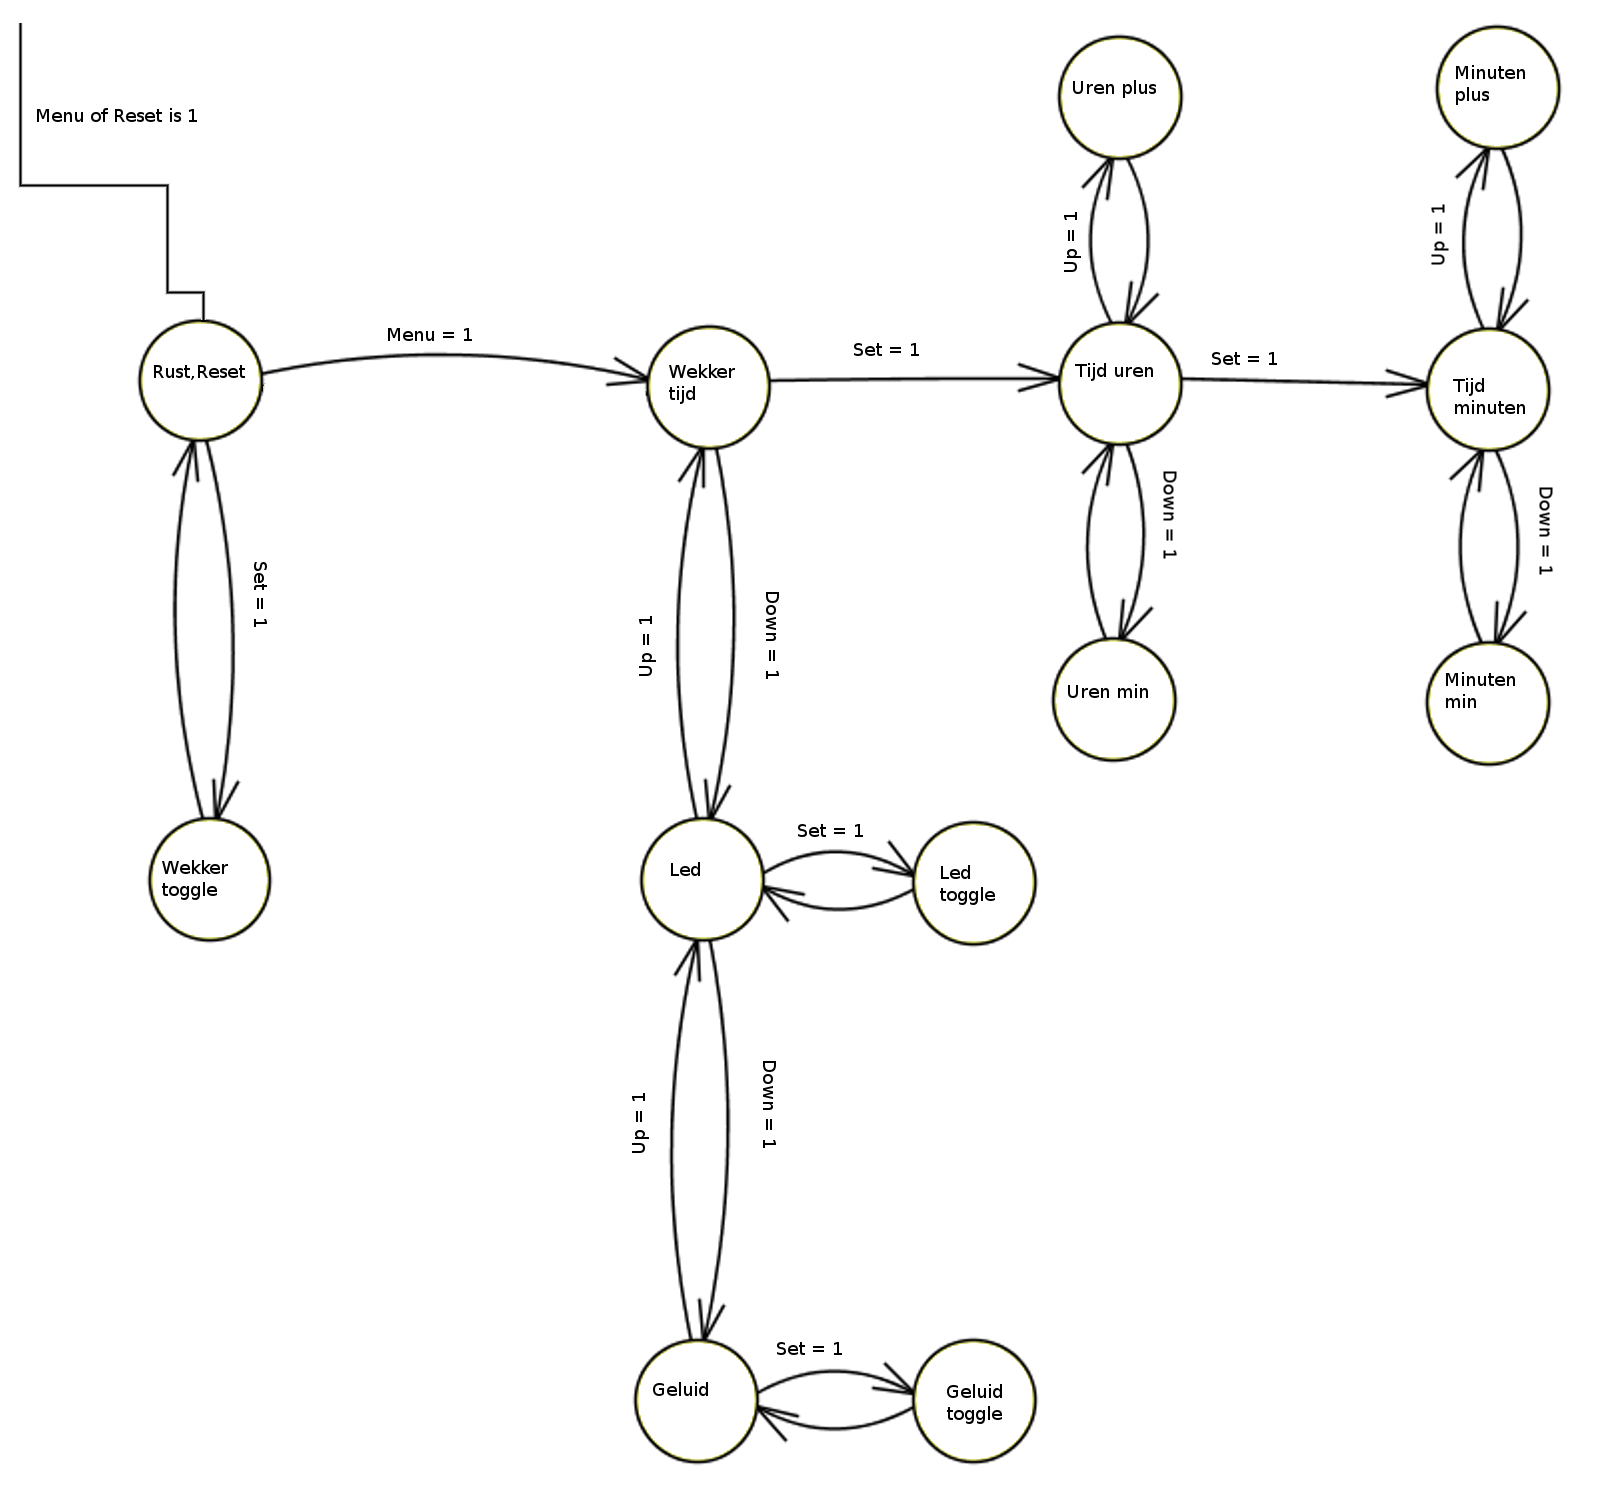
\includegraphics[width=\textwidth,height=\textheight,keepaspectratio]{FSM/controller_fsm.png}
\caption{FSM diagramma van de menu}
\label{fig:FSM_controller}
\end{figure}

\begin{longtable}{|l| p{10cm} |}
\hline
Rust, Reset &
enable ='0' \newline
wekker=wekdata \newline
menu='000' \\ \hline
Wekker toggle &
enable ='1' \newline
wekker[12 down to 0]=wekdata[12 down to 0] \newline
wekker[13]=niet wekdata[13] \newline
menu = menu \\ \hline
Wekkertijd &
enable ='0' \newline
wekker=wekdata \newline
menu = 000 \\ \hline
Led &
enable ='0' \newline
wekker=wekdata \newline
menu = 011 \\ \hline
Led toggle &
enable ='1' \newline
wekker[11 down to 0]=wekdata[11 down to 0]\newline
wekker[12] = niet wekdata[12] \newline
wekker[13] = wekdata[13] \newline
menu = menu \\ \hline
Geluid & 
enable ='0' \newline
wekker=wekdata of een mooi getal code \newline
menu = 100 \\ \hline
Geluid toggle &
enable ='1' \newline
wekker[10 down to 0]=wekdata[10 down to 0] \newline
wekker[11] = niet wekdata[11] \newline
wekker[13 downto 12] = wekdata[13 downto 12] \newline
menu = menu \\ \hline
Uren set &
enable ='0' \newline
wekker=wekdata \newline
menu = 001 \\ \hline
Uren plus &
enable ='1' \newline
wekker=wekker+1 \newline
menu =menu \\ \hline
Uren min &
enable ='1' \newline
wekker=wekdata-1 \newline
menu = menu \\ \hline
Minuten set &
enable ='0' \newline
wekker=wekdata \newline
menu = 010 \\ \hline
Minuten plus &
enable ='1' \newline
Wektijd=wekdata+1 \newline
menu = menu \\ \hline
Minuten min &
enable ='1' \newline
wekker=wekdata-1 \newline
menu = menu \\ \hline
\caption{Uitgangen binnen de state van de controller} 
\label{tab:states_controller}
\end{longtable}

\subsection{VHDL code}
De code voor de controller van de wekker is te vinden in \cref{Ap:code_controller}. Voor de overzicht en het modular opbouwen is de code in vier blokken geschreven.
\begin{itemize}[nolistsep]
\item De top entity met de port map \cref{code:controller_ent,code:controller_beh}.
\item De menu opzichzelf hierin zit het echt logica in verwerkt te vinden in \cref{code:menu_ent,code:menu_beh}.
\item Het gebruikte geheugen element voor de opslag van 14 bits te vinden in \cref{code:geheugen_ent,code:geheugen_beh}.
\item De gebruikte buffer is te vinden in \cref{code:buffer_ent,code:buffer_ent}. De buffer regelt het ingangssignaal, en zorgt ervoor dat er maar 1 klokperiode lang een hoog signaal gelezen word
\end{itemize}
Voor het testen van de code zijn er testbenches gemaakt welke te vind zijn in \cref{code:tb_controller,code:tb_menu,code:tb_geheugen,code:tb_buffer}
\section{Resultaten}
Als eerste is een test gedaan door de VHDL code te simuleren met \emph{Modelsim}. Toen bleek dat dit een goed resultaat afleverde, is de code gesynthetiseerd, en is daarmee nog een simulatie gedaan. Toen bleek dat ook dit een goed resultaat afleverde, is de VHDL code geextraheerd, en deze code is opnieuw gesimuleerd. Vervolgens is nog een switch-level simulatie uitgevoerd, en hierna werd de code stabiel verklaard.

\subsection{Simulatie}

\subsection{Conclusie en discussie}
De controller werkt op alle gesimuleerde niveau's correct en naar verwachting. De minimale klok periode bedraagt 60ns om gliches te voorkomen bij het optellen en aftrekken van uren en minuten. De controller maakt op dit moment gebruik van 9088 transitoren waarvan er voor de daadwerkelijke schakelingen slechts 2914 worden gebruikt. De controller maakt op dit moment nog gebruik van het binary tel systeem met machten van twee echter bleek dat voor de lcd scherm BCD veel beter werkt dit moet nog worden ge\"{i}mplementeerd.



\chapter{Alarm}
\section{Inleiding}
In de alarm module wordt een led aangestuurd, die 15 minuten voor de ingestelde tijd in de main controller begint met branden en steeds feller wordt naarmate de tijd verstrijkt. Als de huidige tijd gelijk is aan de ingestelde tijd brandt de led op z'n felst en gaat er een geluid af, totdat er een knop wordt ingedrukt.

\section{Specificaties}
\subsection{Ingangen}
\begin{itemize}[nolistsep]
\item Klok, standaard input.
\item Reset, standaard input.
\item Tijd-uur, huidige tijd in uren.
\item Tijd-minuut, huidige tijd in minuten.
\item Wekker-uur, uur ingesteld in de main controller.
\item Wekker-min, minuten ingestels in de main controller.
\item Sec, seconde signaal gegenereerd in de DCF controller.
\item Knop, alarm uitschakelen.
\end{itemize}

\subsection{Uitgangen}
\begin{itemize}[nolistsep]
\item PWM-signaal, signaal om de led aan te sturen.
\item Geluid, signaal om een geluid af te laten gaan.
\end{itemize}

\subsection{Gedrag}
Het alarm moet een bepaalde tijd voordat de wekker is ingesteld aangaan, nu gekozen voor 15 minuten.
Er wordt 15 minuten van de ingestelde tijd afgetrokken. Zodra die tijd gelijk is aan de huidige tijd komt er een signaal (licht) aan bij het gedeelte wat voor een pwm signaal zorgt.
In dat gedeelte wordt een pwm signaal gegenereerd dat elke 15 seconde breder wordt. Dit wordt gedaan door in een counter 15 seconde te tellen. Elke 15 seconde wordt de variable "lenght" kleiner. Deze begon op 64 en wordt vergeleken met een andere counter die elke klokflank telt, tot 64. Als de counter groter of gelijk is aan "length" dan is het pwm-signaal hoog. 
Als 15 minuten zijn verstreken na het aangaan van de led, dus de ingestelde tijd is gelijk aan de huidige tijd, brandt de led op z'n felst. Ook zal dan een "geluid" signaal naar '1' gaan. Dit blijft zo totdat de knop wordt ingedrukt of alles wordt gereset.

\chapter{LCD controller}
\section{LCD Controller}
Op de LCD zal de huidige tijd, ingestelde wekkertijd, datum en ingeschakelde functies te zien zijn. Een LCD is daar handig voor omdat het veel ontwerp vrijheid bied. Dat neemt ook mee dat het erg gecompliceerd kan worden. Het LCD dat zal worden gebruikt is van de fabrikant MIDAS, typenummer MC128064B6W-BNMLW~\cite{Datasheet_lcd}. Het betreft een graphical LCD van 128 x 64 pixels met een register die geschreven kan worden. De bibliotheek met characters en de controller om het LCD te schrijven zal extern van deze chip plaatsvinden door middel van een atmega32-16pu~\cite{Datasheet_micro}. Deze keuze is gemaakt omdat voor de characters niet genoeg ruimte is op de chip. De LCD controller op de chip zal dus alleen de inkomende data moeten omzetten naar een positie waarnaar het geschreven moet worden en een bijbehorend character. De layout van het display is al vastgesteld, zodat de posities alvast bekend zijn.  Zie voor de layout afbeelding \ref{fig:lcdlayout}.  \\

\begin{figure}
  \centering
     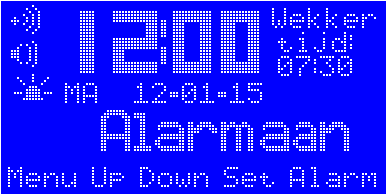
\includegraphics[angle = 0, scale= 1]{Figuren/LCD/voorbeeld_lcd.png}
       \caption{LCD layout}
\label{fig:lcdlayout}
\end{figure}

\section{Specificaties}

\begin{center}
\label{table:uitgangen}
\begin{tabular}{| l | l | p{4.5cm} |}
\hline
\textbf{Naam} & \textbf{Type} & \textbf{Functie} \\ \hline
clk           				& in std$\_$logic           									& Klok             \\ \hline
reset         			& in std$\_$logic           									& Reset            \\ \hline
ready					& in std$\_$logic 											&  \\ \hline
uren						&in std$\_$logic$\_$vector(5 downto 0) 		&data signaal met actuele uren afkomstig van DCF \\ \hline
minuten				&in std$\_$logic$\_$vector(6 downto 0) 		&data signaal met actuele minuten afkomstig van DCF \\ \hline
dagvdweek			&in std$\_$logic$\_$vector(2 downto 0)			&data signaal met de actuele dag afkomstig van DCF\\ \hline
dagvdmaand		&in std$\_$logic$\_$vector(5 downto 0) 		&data signaal met de actuele dag van de maand afkomstig van DCF \\ \hline
maand					&in std$\_$logic$\_$vector(4 downto 0) 		&data signaal met de actuele maand afkomstig van DCF  \\ \hline
jaar						&in std$\_$logic$\_$vector(7 downto 0)	 		&data signaal met het actuele jaar afkomstig van DCF  \\ \hline
dcf$\_$debug		&in std$\_$logic 												&signaal afkomstig van het dcf component en weergeeft of het DCF signaal ontvangen wordt of niet \\ \hline
menu					&in std$\_$logic$\_$vector(2 downto 0)			&data signaal die de actuele menu state weergeeft \\ \hline
alarm 					&in std$\_$logic												&buffer signaal dat weergeeft of alarmfunctie in of uitgeschakeld is\\ \hline
geluid$\_$signaal 		&in std$\_$logic 		 										&buffer signaal dat weergeeft of geluidsfunctie in of uitgeschakeld is \\ \hline
licht$\_$signaal 	&in std$\_$logic 		 										&buffer signaal dat weergeeft of lichtfunctie in of uitgeschakeld is  \\ \hline 
wektijd$\_$uren 	& in std$\_$logic$\_$vector(5 downto 0)		&data signaal met ingestelde wektijd uren \\ \hline 
wektijd$\_$min 	&in std$\_$logic$\_$vector(6 downto 0) 		&data signaal met ingestelde wektijd minuten \\ \hline 
data$\_$out 		&out std$\_$logic$\_$vector(6 downto 0) 		&data signaal dat de x,y,c informatie doorgeeft aan de microcontroller \\ \hline 
clk$\_$out 			&out std$\_$logic 		 										&clock om microcontroller clock mee te synchroniseren \\ \hline 
\end{tabular}
\end{center}

\newpage
\begin{figure}
  \centering
     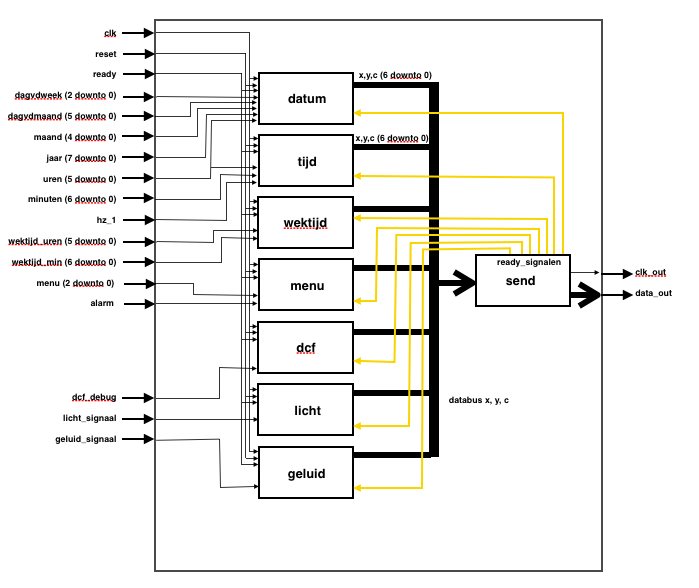
\includegraphics[angle = 0, scale= 0.5]{verslag_schemas/toplevel_entity.png}
       \caption{Toplevel Entity}
\label{fig:lcdtoplevel}
\end{figure}
\newpage

\subsection{Gedrag}
De LCD controller zal na de reset alle informatie die hij binnen krijgt omzetten naar een karakter met bij behorende x en y positie en wegschrijven naar de microprocessor van de LCD. Daarna zal de controller alleen de data die veranderd op de ingangen omzetten en  wegschrijven naar de microprocessor om tijd en onnodige acties te besparen. \\
Het verzenden van de x,y en c gaat door een data signaal van 7 bits samen met een clock$\_$out. Een neergaande klokflank geeft aan dat de data klaar staat om te verzenden zodat er op de opgaande klokflank kan worden gesampled. Zo zal eerst de x, daarna de y en als laatste de c worden verzonden. Het versturen van een karakter duurt dus 3 klokslagen van de clock$\_$out. een klokslag van de clock$\_$out is gelijk aan 2 klokslagen van de ingaande clk. 

\section{Functionaliteit}
De systemen links (datum, tijd, etc)  zorgen per stuk voor het ontvangen van de inkomende informatie en het omzetten naar een x,y positie met een karakter. De x,y en de c zal op de uitgang van het component worden gezet. 
Het component send$\_$buffer is een MUX en zorgt voor het uitlezen van de x,y en c en zal door middel van de ready signalen aangeven welk signaal hij heeft uigelezen en naar de zender heeft verstuurd. Zodra de ready laag wordt, weet het desbetreffende component dat de data is uitgelezen en zal daarna nieuwe data klaar zetten. 
Nadat de mux de data naar de zender heeft gebufferd, zal de zender de signalen een voor een door  verzenden naar de microcontroller. Tegelijkertijd zal de zender een clock$\_$out geven, zodra de clock laag wordt staat de data klaar, zodat op de opgaande klokflank de data vanaf de chip kan worden uitgelezen. 

\section{Subsystemen LCD}

\subsection{Datum}
\subsubsection{Gedrag}
Na een reset of \'e\'en keer per dag om 12 uur middernacht zal het datum component de data voor de nieuwe datum verzenden naar de zend buffer. De inkomende data is in het binary coded decimal (bcd) formaat. Eerst zal hij de dag van de week doorgeven, daarna de dag van de maand, de maand en daaropvolgend het jaartal. Dat allemaal sequentieel, getriggert op de neergaande klokflank van de ready$\_$buf. 

\begin{figure}
  \centering
     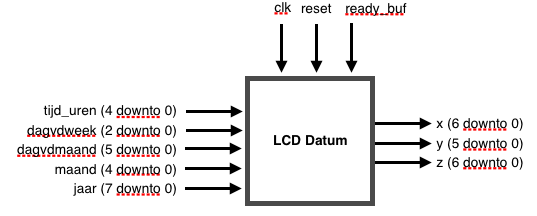
\includegraphics[angle = 0, scale= 0.75]{verslag_schemas/datum_entity.png}
       \caption{Entity datum}
\label{fig:datumentity}
\end{figure}


\subsubsection{Functionaliteit}
Het component werkt met een finite state machine (FSM) waarin de characters worden klaargezet en een counter genaamd positie wordt aangestuurd met daarnaast een apart process om de juiste input te bepalen afhankelijk van de counter. \\
Na de reset zal de FSM in de selectdata state starten en positie op 0 worden gezet. 
In het aparte process zal de de data$\_$buf worden gekoppeld aan de input die hoort bij positie=0 en zal de x en y bepaald worden. 
 In selectdata zal  afhankelijk van de counter (in dit geval 0) worden bepaald of de dag van de week of de getallen van de datum moet worden geschreven. Bij positie=0 zal het karakter van de dag van de week (in state cdvdw) worden klaargezet. Het karakter wordt bepaald door de waarde die op de data$\_$buf staat. Op de neergaande klokflank van het ready$\_$buf signaal zal de FSM terug gaan naar de state selectdata en zal er bij positie 1 worden opgeteld. Daardoor zal hierna het eerste getal van de datum worden geschreven. Dit zal zich herhalen tot positie =7, daarna zal hij naar de rust stand gaan en is de datum geschreven. \\
 Als het middernacht is, dus tijd$\_$uren = '00000', zal er ook een nieuwe datum worden klaargezet. Zodra de positie 7 is zal de machine in state selectdata blijven hangen totdat de tijd$\_$uren ongelijk is aan "00000". Dit om te voorkomen dat het component een uur lang onnodig data blijft verzenden. 


\subsubsection{FSM}
\begin{figure}
  \centering
     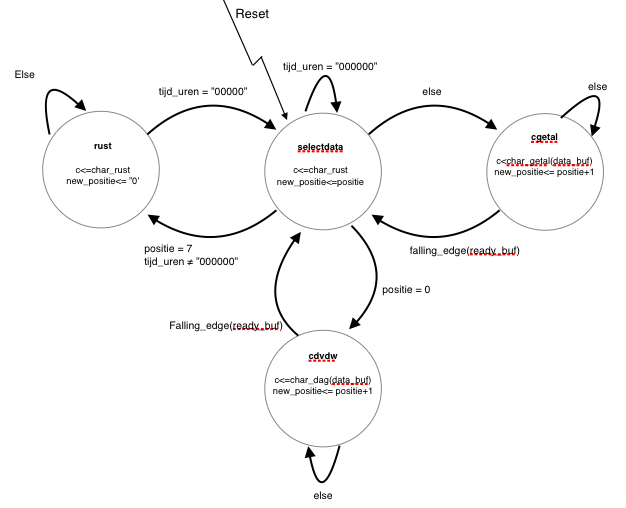
\includegraphics[width=15cm]{verslag_schemas/datum_fsm.png}
       \caption{FSM Datum}
\label{fig:lcddatumfsm}
\end{figure}

\subsubsection{VHDL code}
Zie \ref{code:ent_datum} voor de entity code. \\
Zie \ref{code:beh_datum} voor de behavioural code.\\
Zie \ref{code:tb_datum} voor de testbench die is gebruikt.
\subsubsection{Simulaties}
Zie \ref{fig:sim_datum_behavioural} voor de simulatie van de behavioural code. \\
Zie \ref{fig:sim_datum_circuit} voor de simulatie van het gesynthetiseerde circuit. 
De simulaties zijn uitgevoerd met een clock van 2000ns.  Er is getest tot 300k ns, zie de testbench in \ref{code:tb_datum} voor meer informatie.

\subsubsection{Resultaten}
Uit de simulaties is gebleken dat het circuit doet waarvoor het is ontworpen.

\subsection{Tijd en Wektijd}

\subsubsection{Gedrag}
Na een reset of bij het veranderen van de minuten zal de entity tijd data gaan verzenden. De data die verzonden wordt bevat informatie over welk character geprint moet worden en zijn positie. De characters die moeten worden verzonden worden bepaalt aan de hand van de minuten en uren die de entity in gaan. Dit zal altijd op de volgende volgorde gaan: tientallen uren, eentallen uren, tientallen minuten en als laatste eentallen minuten. Ook zal de module bij een opgaande flank van het \'e\'en Hz signaal de dubbele punt tussen de uren en minuten aan of uit zetten.\\
Het component wektijd verzend dezelfde informatie naar het LCD, alzij het op een andere positie. De wektijd zal beginnen met verzenden op het moment dat de wektijd wordt aangepast in het menu. De volgorde van de

\subsubsection{Functionaliteit}
Het component werkt volgens het Moore principe. Om de seconde wordt een nieuw character naar het LCD gestuurd. Dit character is voor de dubbele punt tussen de uren en minuten. Als er een minuut om is dan zal de nieuwe tijd naar het LCD worden verzonden.

\subsubsection{FSM}

\subsubsection{VHDL code}

\subsubsection{Simulaties}

\subsubsection{Testen}

\subsubsection{Resultaten}

\subsubsection{Discussie}

\input{LCD_controller/menu}
\input{LCD_controller/dcf}
\input{LCD_controller/geluidenlicht}
\subsection{Zender}

\subsubsection{Gedrag}
De zender zorgt ervoor dat de x, y en c van de verschillende componenten bij de microcontroller komen. Dit doet het component door een x, y en c waarde in te nemen, en deze vervolgens in de goede volgorde op de uitgang te zetten. De zender zal altijd beginnen met de x op de uitgang te zetten. Daarna zal de zender het signaal clk\_out omlaag brengen, om op de volgende klokslag dit signaal weer hoog te maken. Op de volgende klokflank zal clk\_out weer omlaag gebracht worden en y op de uitgang gezet worden. Daarna zal clk\_out weer hoog worden en zal het geheel nog herhaald worden voor de c. Nadat deze reeks is verzonden zal er bekeken worden of het volgende blok data wil verzenden. Als dit het geval is dan zal deze data verzonden worden. Mocht dat niet het geval zijn dan wordt dat blok overgeslagen en gaat de zender naar het volgende blok.

\subsubsection{Functionaliteit}
Het doel van de zender is om de data die de afzondelijke componenten willen verzenden, goed naar de microcontroller worden verzonden. Dit moet goed door de microcontroller begrepen worden. Daarom zal de volgorde van de verzonden data altijd hetzelfde zijn. Tussen twee verschillende blokken data zit altijd een beetje extra tijd. Dit is minimaal 1 klokslag. Hierdoor weet de microcontroller dat de vorige transmissie afgelopen is en dat het volgende blok weer bij de x begint.\\
Alle blokken kunnen tegelijk verzenden. De blokken moeten namelijk op een ready signaal wachten van de zender. Vervolgens selecteert de verzender via een bus naar welk blok wordt gekeken om data te verzenden. Mocht dit blok niks te verzenden hebben dan zal de c van dat blok op ''0000000'' staan. Hierdoor weet de zender dat het niks hoeft te verzenden en zal naar het volgende blok gaan.

\subsubsection{FSM}
De FSM van de zender is te vinden in \ref{fig:fsm_zender}
\begin{figure}[h!]
	\center
	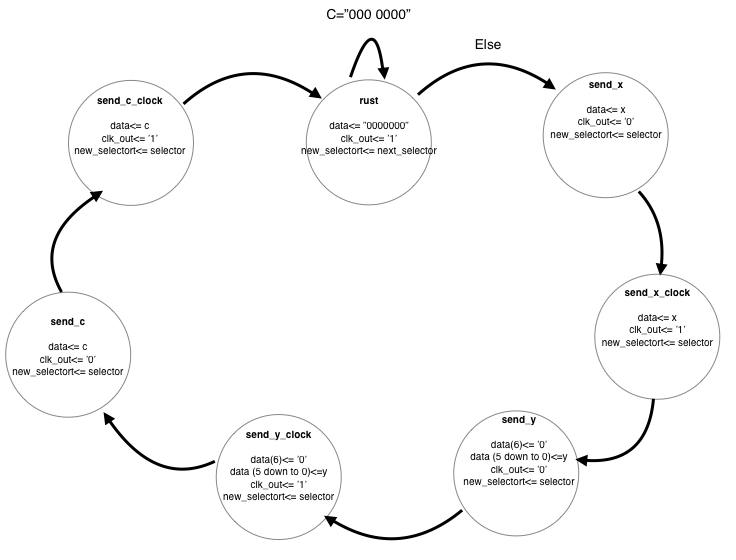
\includegraphics[width = 15cm]{Figuren/LCD/fsm_sender.png}
	\caption{FSM van component zender}
	\label{fig:fsm_zender}
\end{figure}

\subsubsection{VHDL code}
De vhdl code van de zender is opgedeeld in twee stukken, namelijk een send control en een send bus. Deze twee zijn vervolgens met een structural behaviour bij elkaar gevoegd. De code van de send control is te vinden in \ref{code:ent_send_control} en \ref{code:beh_send_control}. De code voor de send bus is te vinden in \ref{code:ent_send_bus} en \ref{code:beh_send_bus}. De top structure is te vinden in \ref{code:ent_send_top} en \ref{code:struc_send_top}.

\subsubsection{Simulaties}
De simulatie van de gehele zender is te vinden in \ref{fig:sim_send_top}. Hierin is goed te zien dat ready voor elk blok apart omhoog gaat en dat het blok voor blok behandeld wordt. Deze simulatie is gedaan met de testbench in \ref{code:tb_send_top}.

\subsubsection{Resultaten}
De simulatie is zoals te verwachten valt. Hierdoor kan geconcludeert worden dat de zender naar behoren werkt.

\subsection{VHDL code}
Zie \ref{code:ent_lcd_top} voor de entity code. \\
Zie \ref{code:beh_lcd_top} voor de behavioural code.\\
Zie \ref{code:tb_lcd_top} voor de testbench die is gebruikt.

\section{Simulatie}
Zie \ref{fig:sim_lcdtop} voor de simulatie van de behavioural code. \\

\section{Testen}
Tijdens het testen van verschillende subcircuits zijn veel dingen fout gegaan. Vaak waren de circuits dan ook wel goed, maar was de testbench niet correct. Zo hebben we in het begin met een te hoge clock frequentie getest, maar ook met signalen die niet lang genoeg hoog bleven. \\
Het systeem is ook getest op een Altera FPGA bord. Eerst dachten we dat het niet werkte, maar achteraf bleek dat, wat best logisch is,  het systeem zodanig snel werkt dat wij zelf het niet konden waarnemen. Door de klok te pulsen met een button konden we zien dat het systeem weldegelijk correct werkt.

\section{Resultaten}
De resultaten zijn goed. Het systeem heeft 2 errors in de switch level simulatie. Dat heeft te maken met de testbench waarin een situatie wordt gecre\"eerd die zich nooit zal voordoen. Dat maakt dus niks uit.

\subsection{Conclusie en discussie}
De controller werkt naar verwachting. Omdat vanwege tijdgebrek en gestelde prioriteiten de microcontroller nog niet af is voor het LCD kan nog niet worden getest of het systeem ook daarmee goed functioneerd. Al verwachten wij, omdat de simulaties en de test op de FPGA positief zijn, dat het kan gaan werken.\\


\chapter{Results for total design}
text text text...

\chapter{Plan voor het testen van de chip}
%Moet het gaan over het testen van de daadwerkelijke gemaakte chip in Q4 of moet het gaan over het testen op de fpga
Voor het testen zijn een aantal momenten in het proces waarop getest wordt. Zo wordt elk module getest in een simulatie in Modelsim. Hieruit kan opgemaakt worden wat het verwachte gedrag is. Maar een simulatie is niet alles. Daarom kan een module ook nog getest worden door middel van een FPGA te programmeren. De uiteindelijke chip zal getest worden met een logic analyzer en natuurlijk door te kijken of de chip de gewenste output geeft.
\section{FPGA bord}
Het bord dat gebruikt kan worden is een Altera FPGA bord. Dit bord komt met eigen software genaamt Quartus. Deze software kan gebruikt worden om de gemaakte VHDL code om te zetten in een bitstream file en vervolgens het FPGA bord te programmeren. Door de VHDL code op een FPGA te programmeren kan worden geverifieerd of de code het gedrag vertoont wat verwacht wordt. Door simulatie is dit namelijk niet altijd helemaal te zien. Mocht op de FPGA een fout ontdekt worden, dan zal de code hierop aangepast worden en zal de code opnieuw gesimuleerd worden.
\section{Logic Analyzer}
De gemaakte chip zal in Q4 worden getest. De chip zal eerst op een logic analyzer worden aangesloten. De analyzer die gebruikt zal worden is een LA-5580.


\chapter{Voortgang van het project}

\section{Inleiding}
Bij dit project zijn er vaak weinig resultaten, totdat het bijna afgelopen is. 
Dit is een van de redenen dat voor een wake-up light gekozen is.
Een wekker zelf is relatief makkelijk te maken. 
Er zijn echter ook een hele hoop extra features die in een wekker geimplementeerd kunnen worden. 
Op deze manier is dus een werkend resultaat relatief snel geproduceerd, en kunnen daarna naar gelang extra toepassingen toegevoegd worden. 
Dit is goed voor het moreel in de groep, aangezien een werkend product al heel snel gerealiseerd is.
Hierdoor is er ook meer aansporing om meer toepassingen te implementeren, omdat er al een werkend geheel is. 
In het ergste geval is er geen extra feature.
Daarnaast, als uiteindelijk bleek dat de planning te krap was, kunnen er features geschrapt worden, en is er nog steeds een werkend product. 
Onder andere dit maakt een wake-up light zeer aantrekkelijk om te maken.

\section{Werkverdeling}
De eerste twee weken werd er gewerkt aan een module-opdracht, in de vorm van een opwarmertje


\section{Samenwerking binnen de groep}

\section{Afspraken binnen de groep}


\chapter{Conclusie}



%% Use letters for the chapter numbers of the appendices.
\appendix

\chapter[VHDL code]{Vhdl code van de controller}
\section{Top level entity}
\scriptsize 
 \lstinputlisting [style= VHDL]{vhdl/controller/controller.vhd}
 \normalsize
\label{code:controller_ent}
\section{Behavioural VHDL code controller}
\scriptsize 
 \lstinputlisting [style= VHDL]{vhdl/controller/controller_beh.vhd}
 \normalsize
\label{code:controller_beh}
\section{Menu entity}
\scriptsize 
 \lstinputlisting [style= VHDL]{vhdl/controller/menu-ent.vhd}
 \normalsize
\label{code:menu_ent}
\section{Behavioural VHDL code menu}
\scriptsize 
 \lstinputlisting [style= VHDL]{vhdl/controller/menu-behaviour.vhd}
 \normalsize
\label{code:menu_beh}
\section{Memory}
\scriptsize 
 \lstinputlisting [style= VHDL]{vhdl/controller/geheugen.vhd}
 \normalsize
\label{code:gehuegen_ent}
\section{Behavioural VHDL memory}
\scriptsize 
 \lstinputlisting [style= VHDL]{vhdl/controller/geheugen-behaviour_fsm.vhd}
 \normalsize
\label{code:gehuegen_beh}
\section{Entity buffer}
\scriptsize 
 \lstinputlisting [style= VHDL]{vhdl/controller/buffer_ent.vhd}
 \normalsize
\label{code:buffer_ent}
\section{Behavioural VHDL buffer}
\scriptsize 
 \lstinputlisting [style= VHDL]{vhdl/controller/buffer_beh.vhd}
 \normalsize
\label{code:buffer_beh}
\chapter[Simulatie resultaten]{Simulaties resultaten van de controller}
\label{Ap:sim_controller}
\section{Behavoral simulatie}
\begin{figure}[ht!]
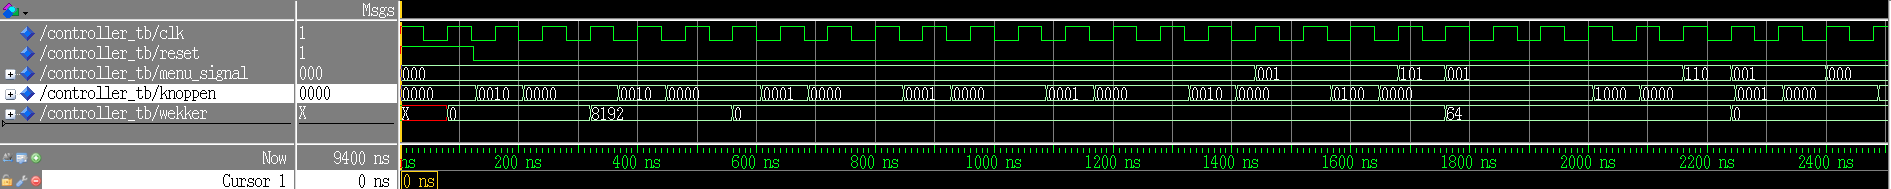
\includegraphics[width=\textwidth,height=\textheight,keepaspectratio]{results/controller/wave0-2_5.png}
\caption{Simulatie van 0 tot 2500ns}
\label{fig:sim_beh_0-2_5}
\end{figure}
\begin{figure}[ht!]
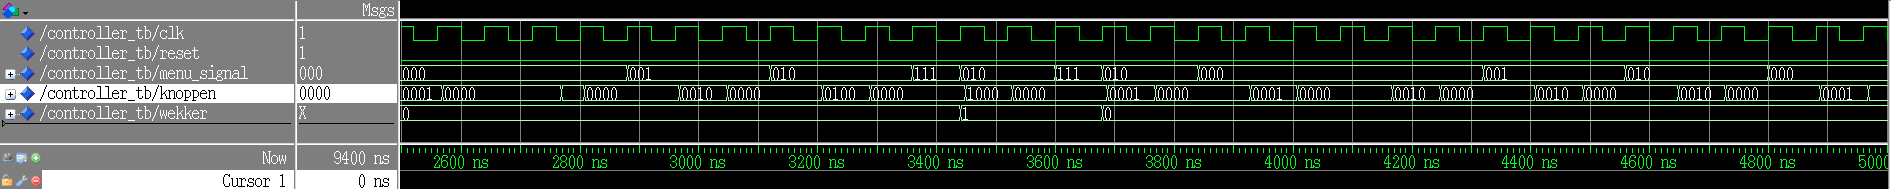
\includegraphics[width=\textwidth,height=\textheight,keepaspectratio]{results/controller/wave2_5-5.png}
\caption{Simulatie van 2500ns tot 5000ns}
\label{fig:sim_beh_2_5-5}
\end{figure}
\begin{figure}[ht!]
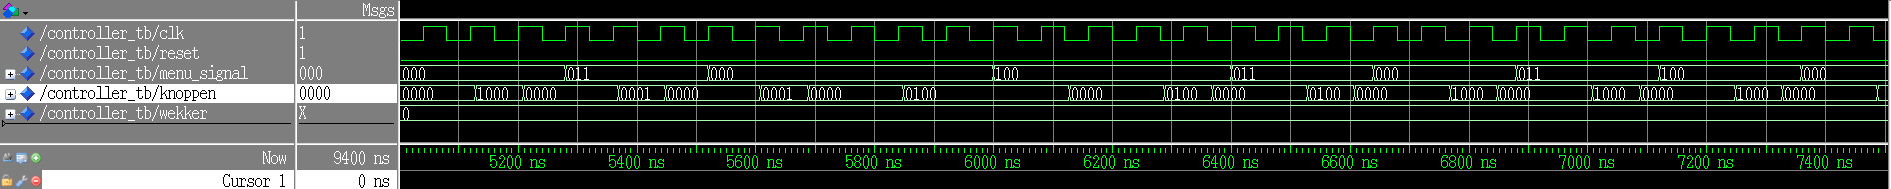
\includegraphics[width=\textwidth,height=\textheight,keepaspectratio]{results/controller/wave5-7_5.png}
\caption{Simulatie van 5000ns tot 7500ns}
\label{fig:sim_beh_5-7_5}
\end{figure}
\begin{figure}[ht!]
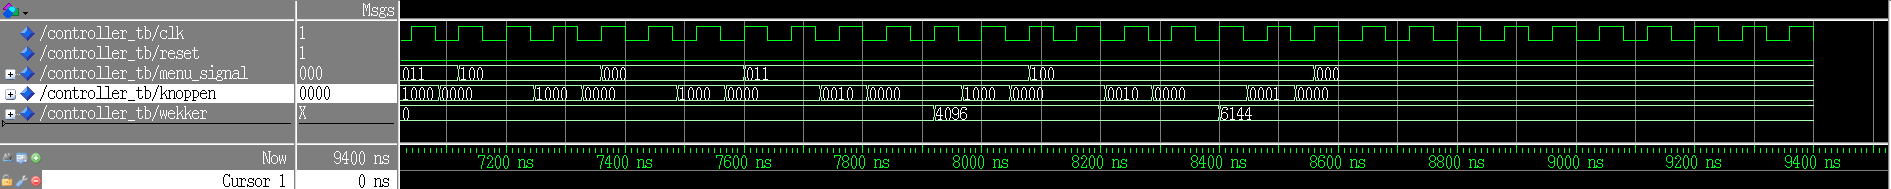
\includegraphics[width=\textwidth,height=\textheight,keepaspectratio]{results/controller/wave7_5-.png}
\caption{Simulatie van 7500ns tot het einde}
\label{fig:sim_beh_7_5-}
\end{figure}
\newpage
\section{Synthesize simulatie}
\begin{figure}[ht!]
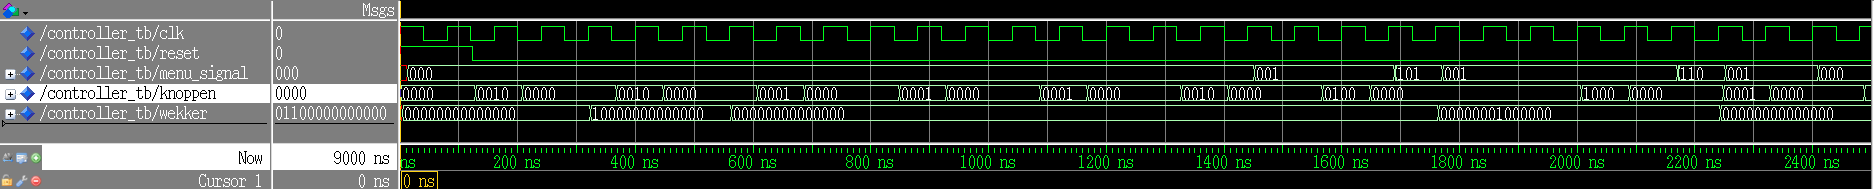
\includegraphics[width=\textwidth,height=\textheight,keepaspectratio]{results/controller/wave0-2_5_syn.png}
\caption{Simulatie van 0 tot 2500ns}
\label{fig:sim_syn_0-2_5}
\end{figure}
\begin{figure}[ht!]
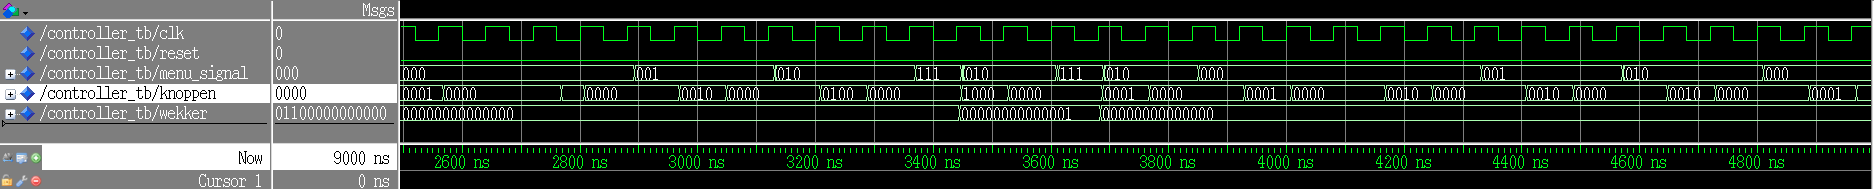
\includegraphics[width=\textwidth,height=\textheight,keepaspectratio]{results/controller/wave2_5-5_syn.png}
\caption{Simulatie van 2500ns tot 5000ns}
\label{fig:sim_syn_2_5-5}
\end{figure}
\begin{figure}[ht!]
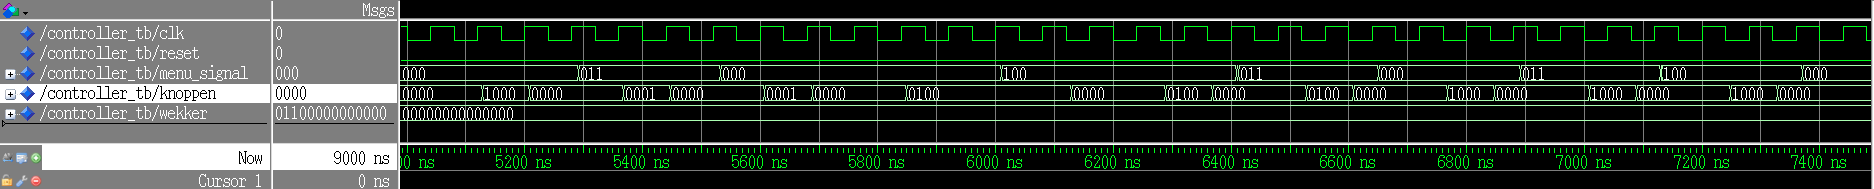
\includegraphics[width=\textwidth,height=\textheight,keepaspectratio]{results/controller/wave5-7_5_syn.png}
\caption{Simulatie van 5000ns tot 7500ns}
\label{fig:sim_syn_5-7_5}
\end{figure}
\begin{figure}[ht!]
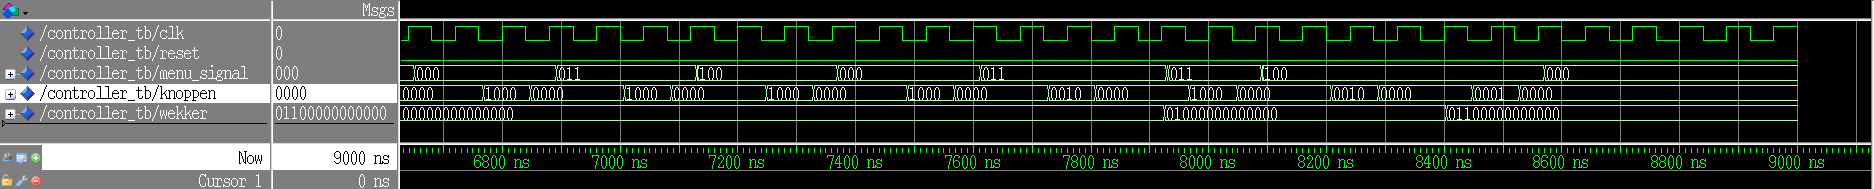
\includegraphics[width=\textwidth,height=\textheight,keepaspectratio]{results/controller/wave7_5-_syn.png}
\caption{Simulatie van 7500ns tot het einde}
\label{fig:sim_syn_7_5-}
\end{figure}
\newpage
\section{Extracted simulatie}
\begin{figure}[ht!]
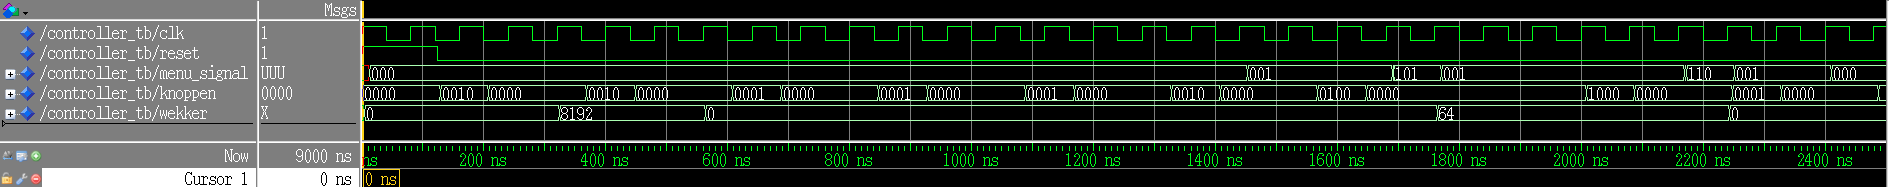
\includegraphics[width=\textwidth,height=\textheight,keepaspectratio]{results/controller/wave0-2_5_ext.png}
\caption{Simulatie van 0 tot 2500ns}
\label{fig:sim_ext_0-2_5}
\end{figure}
\begin{figure}[ht!]
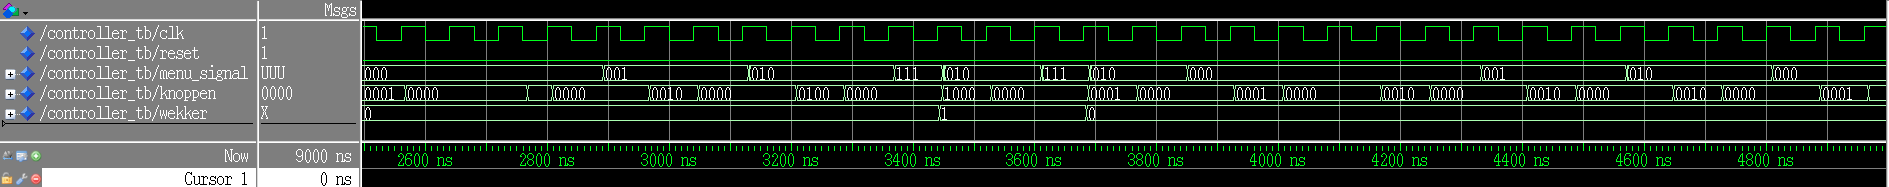
\includegraphics[width=\textwidth,height=\textheight,keepaspectratio]{results/controller/wave2_5-5_ext.png}
\caption{Simulatie van 2500ns tot 5000ns}
\label{fig:sim_ext_2_5-5}
\end{figure}
\begin{figure}[ht!]
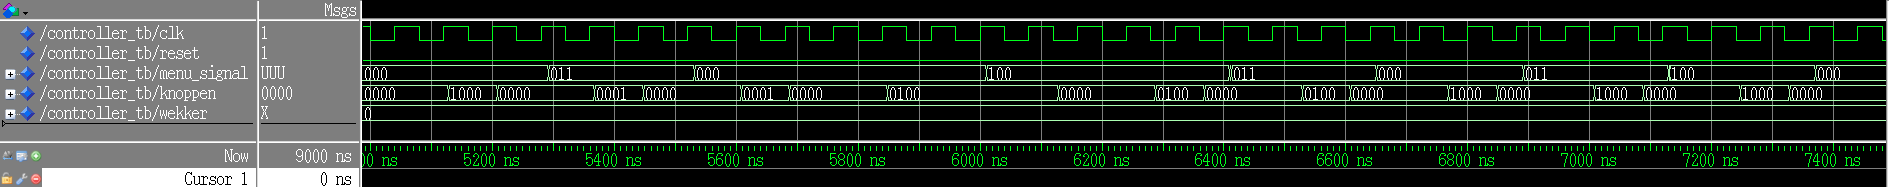
\includegraphics[width=\textwidth,height=\textheight,keepaspectratio]{results/controller/wave5-7_5_ext.png}
\caption{Simulatie van 5000ns tot 7500ns}
\label{fig:sim_ext_5-7_5}
\end{figure}
\begin{figure}[ht!]
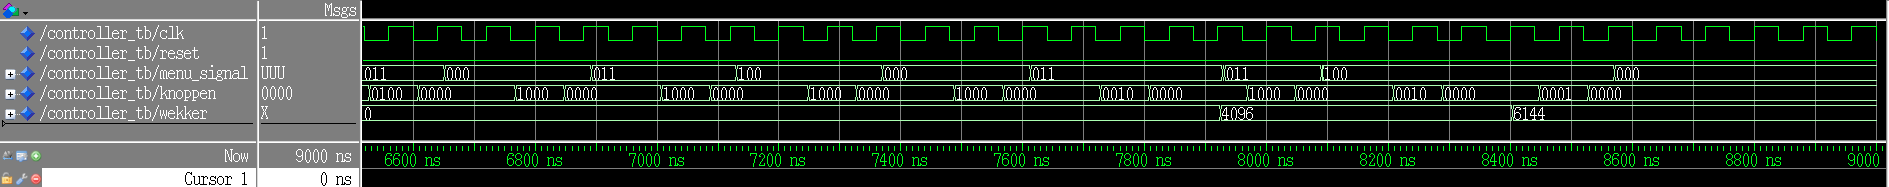
\includegraphics[width=\textwidth,height=\textheight,keepaspectratio]{results/controller/wave7_5-_ext.png}
\caption{Simulatie van 7500ns tot het einde}
\label{fig:sim_ext_7_5-}
\end{figure}
\chapter[VHDL code]{Vhdl code van het alarm}
\label{Ap:code_alarm}
\section{entity alarm-compare}
\scriptsize 
 \lstinputlisting [style= VHDL]{vhdl/alarm/compare.vhd}
 \normalsize
\label{code:ent_alarm_compare}
\section{Behavioural alarm-compare}
\scriptsize 
 \lstinputlisting [style= VHDL]{vhdl/alarm/compare-behaviour.vhd}
 \normalsize
\label{code:beh_alarm_compare}
\section{Top entity alarm}
\scriptsize 
 \lstinputlisting [style= VHDL]{vhdl/alarm/alarm.vhd}
 \normalsize
\label{code:ent_alarm}
\section{Behavioural alarm}
\scriptsize 
 \lstinputlisting [style= VHDL]{vhdl/alarm/alarm-behaviour.vhd}
 \normalsize
\label{code:beh_alarm}
\section{Entity alarm-counter}
\scriptsize 
 \lstinputlisting [style= VHDL]{vhdl/alarm/counter.vhd}
 \normalsize
\label{code:ent_alarm_counter}
\section{Behavioural alarm-counter}
\scriptsize 
 \lstinputlisting [style= VHDL]{vhdl/alarm/counter-behaviour.vhd}
 \normalsize
\label{code:beh_alarm_counter}
\section{Entity alarm-pwm}
\scriptsize 
 \lstinputlisting [style= VHDL]{vhdl/alarm/pwm.vhd}
 \normalsize
\label{code:ent_alarm_pwm}
\section{Behavioural alarm-pwm}
\scriptsize 
 \lstinputlisting [style= VHDL]{vhdl/alarm/pwm-behaviour.vhd}
 \normalsize
\label{code:beh_alarm_pwm}

\bibliography{references}

\end{document}
